\documentclass[letterpaper,12pt]{article}
\usepackage{array}
\usepackage{geometry}
\geometry{letterpaper,tmargin=1in,bmargin=1in,lmargin=1.25in,rmargin=1.25in}
%\renewcommand\headrulewidth{0pt}
%\renewcommand\footrulewidth{0pt}
\usepackage{amsmath}
\usepackage{amssymb}
\usepackage{amsthm}
\usepackage{enumerate}
%\usepackage{harvard}
%\usepackage{setspace}
\usepackage{float,color}
\usepackage[pdftex]{graphicx}
\usepackage{hyperref}
\hypersetup{colorlinks,linkcolor=red,urlcolor=blue}
\theoremstyle{definition}
\newtheorem{theorem}{Theorem}
\newtheorem{acknowledgement}[theorem]{Acknowledgement}
\newtheorem{algorithm}[theorem]{Algorithm}
\newtheorem{axiom}[theorem]{Axiom}
\newtheorem{case}[theorem]{Case}
\newtheorem{claim}[theorem]{Claim}
\newtheorem{conclusion}[theorem]{Conclusion}
\newtheorem{condition}[theorem]{Condition}
\newtheorem{conjecture}[theorem]{Conjecture}
\newtheorem{corollary}[theorem]{Corollary}
\newtheorem{criterion}[theorem]{Criterion}
\newtheorem{definition}[theorem]{Definition}
\newtheorem{derivation}{Derivation} % Number derivations on their own
\newtheorem{example}[theorem]{Example}
\newtheorem{exercise}[theorem]{Exercise}
\newtheorem{lemma}[theorem]{Lemma}
\newtheorem{notation}[theorem]{Notation}
\newtheorem{problem}[theorem]{Problem}
\newtheorem{proposition}{Proposition} % Number propositions on their own
\newtheorem{remark}[theorem]{Remark}
\newtheorem{solution}[theorem]{Solution}
\newtheorem{summary}[theorem]{Summary}
%\numberwithin{equation}{section}
\bibliographystyle{aer}
\newcommand\ve{\varepsilon}
\newcommand\boldline{\arrayrulewidth{1pt}\hline}


\begin{document}

\begin{flushleft}
   \textbf{\large{Problem Set \#3}} \\
   MACS 40000, Dr. Evans \\
   Alexandre Sollaci
\end{flushleft}

\vspace{5mm}

\noindent\begin{enumerate}
   \item \textbf{Fitting elliptical disutility of labor to CFE function}
 	\begin{enumerate}[(a)]
 	\item ]In the CFE case, we have
 	\[ v'_{cfe}(l) = (1-l)^{\frac{1}{\theta}} .\]
 	In the elliptical case, 
 	\[ v'_{elp}(l) = b\left[1 - (1-l)^{\mu}\right]^{\frac{1-\mu}{\mu}} (1-l)^{\mu - 1}\]
 	\item My estimates were $b = 0.501$ and $\mu = 1.554$. The plot of the two marginal utilities can be found in figure 1.
 	\end{enumerate}
	
	\item \textbf{Checking feasibility in the steady-state}
	
	\begin{enumerate}[(a)]
	\item The consumption constraint is violated. Specifically, $c_1 < 0$.
	\item Similarly to the case above, the consumption constraint is violated once more. This time $c_2 < 0$.
	\item In this case, none of the constraints are violated.
	\item Once again, none of the constraints are violated.
	\item As a thumb rule, high values for the labor supply and low (but positive) values for savings will not violate any of the constraints.
	\end{enumerate}
	
	\item \textbf{Solve for the steady-state equilibrium}
	
	\paragraph{Note} Solving for the steady state simply using Python's \texttt{fsolve} was not yielding good results. The solver would frequently produce error messages or converge to ``weird" solutions. I thus adopted the approach discussed in class, where I first guess values for the wage and interest rate, solve for the savings and labor supply of agents and review my guess based on those results. The results aren't perfect, but are a significant improvement.
	\begin{enumerate}[(a)]
	\item The steady state values are
	\begin{verbatim}
'C_ss': 5.2027943970284936,
 'EulErr_ss': array([ 43.67343285, -47.03973973, -13.99275263, ...,   
 0.39490644, 0.36211146,   1.37557797]),
 'K_ss': 3.1406960619335775,
 'L_ss': 9.0752320735278698,
 'RCerr_ss': 6.6613381477509392e-16,
 'Y_ss': 6.2598885230062384,
 'b_ss': array([ 0.06096118,  0.24363708,  0.38449945,  0.45263983, 
         0.49885816, 0.50532795,  0.47201603,  0.36055309,  
         0.16220331]),
 'c_ss': array([ 0.34255851,  0.24285223,  0.35061617,  0.47419286, 
         0.55449917, 0.59131538,  0.64163118,  0.69002686,  
         0.71986051,  0.59524153]),
 'n_ss': array([ 0.9,  0.9,  0.9,  0.9,  0.97535084, 0.93159477, 
         0.94988017,  0.910338  ,  0.87284007,  0.83522823]),
 'r_ss': 0.36102406432043321,
 'ss_time': 0.0036620983482862357,
 'w_ss': 0.4483552053531471
	\end{verbatim}
	\item The distribution of consumption and savings is in figure 2; the distribution of labor supply is in figure 3.
	\item When $\alpha$ drops to 0.25, wages increase, since the marginal product of labor has increased. The increase in wages increases the labor supply, increasing $L$. It also makes consumers richer, so consumption increases and so does aggregate production. Savings drop as a higher fraction of consumer's wealth comes from labor. Despite the decrease in $\alpha$, making capital less valuable for production, the increase in $L$ and in total production end up increasing the marginal product of capital, thus increasing the interest rate as well. 
	
	Figures 4 and 5 show the new distributions of savings, consumption and labor supply. The new steady state values are as below:
	\begin{verbatim}
	'w_ss': 0.52105888806113176
	'r_ss': 0.40894742665033246
	 'b_ss': array([-0.02959289,  0.20073477,  0.26308021,  0.30275722,
	         0.32954978, 0.3392603 ,  0.34118109,  0.28831096,  
	         0.18341839]),
 'c_ss': array([ 0.54908112,  0.22652341,  0.53882572,  0.58498361, 
         0.60998991, 0.63403627,  0.60577184,  0.68919233, 
          0.70573886,  0.72549038]),
 'n_ss': array([ 0.99698564,  0.9 ,  0.99620445,  0.99235357,  
         0.98447736, 0.97681524,  0.9 ,  0.95343747,  
         0.92684776,  0.89637376])
	\end{verbatim}
	\end{enumerate}
	
	\item \textbf{Solve for the non-steady-state equilibrium time path}
	
	As mentioned in question 3, finding the solution to the system of Euler equations was troublesome. This was also an issue for the time path iteration. Although the code runs, to solver keeps going to infeasible points. Curiously, this only happens when it tries to solve simultaneously for savings and labor supply (everything works fine if I feed in a vector of zeros as the labor Euler errors).
	
	In the code that comes with this solution, I have commented the last line (\# 149), which would produce everything asked for in the question. Since the results are obviously wrong (as mentioned, I get corner solutions), I omit the figures for this part.
\end{enumerate}


\section*{Figures}

\begin{figure}[h!]
	\centering
	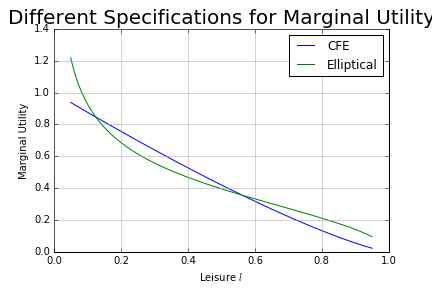
\includegraphics[scale=.8]{code/images/utility_leisure}
	\caption{Marginal utility of leisure in CFE and Elliptical specifications.}
	\end{figure}

\begin{figure}[h!]
	\centering
	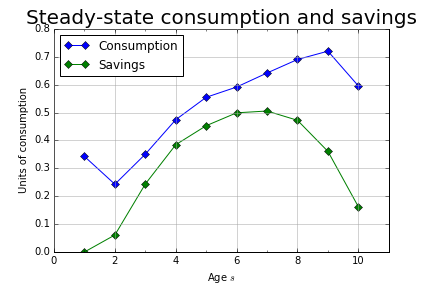
\includegraphics[scale=.8]{code/images/SS_bc}
	\caption{Distribution of consumption and savings in steady state.}
	\end{figure}
	
	\begin{figure}[h!]
	\centering
	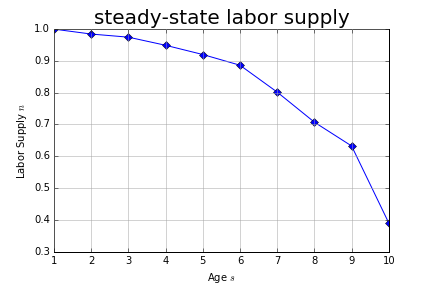
\includegraphics[scale=.8]{code/images/SS_n}
	\caption{Distribution of labor supply in steady state.}
	\end{figure}
	
	\begin{figure}[h!]
	\centering
	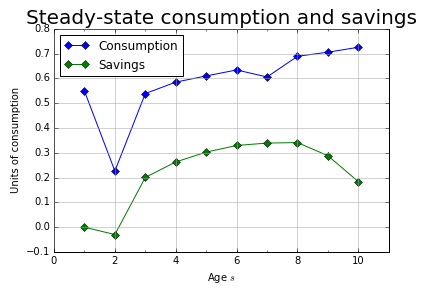
\includegraphics[scale=.8]{code/images/SS_bc2}
	\caption{Distribution of consumption and savings in steady state when $\alpha = 0.25$.}
	\end{figure}
	
	\begin{figure}[h!]
	\centering
	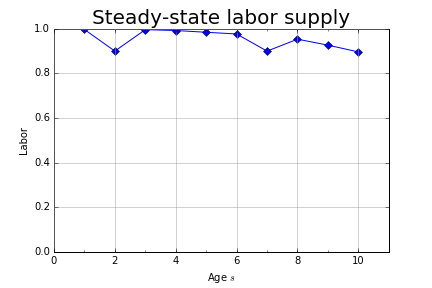
\includegraphics[scale=.8]{code/images/SS_n2}
	\caption{Distribution of labor supply in steady state when $\alpha = 0.25$.}
	\end{figure}

\end{document}





